% =====================================================================
% RBL-5 -- SWT301 Research-Based Learning, Summer 2026
% Group SE1916-G2
%
% FORMAT: EAI FISAT 2026 house style -- Springer LNCS.
%   Required by the course; the paper is NOT submitted to the conference.
%   Format .... Springer LNCS (single column, llncs.cls)
%   Length .... full paper 12-15 pp (short 6-11 pp), excl. refs
%   Language .. English   Review model: single-blind (author names VISIBLE)
%
% llncs.cls and splncs04.bst are on CTAN (CC BY 4.0) and ship with MiKTeX and
% TeX Live, so no manual template download is needed:  https://ctan.org/pkg/llncs
%
% Build:  pdflatex main -> bibtex main -> pdflatex main -> pdflatex main
%   (or)  latexmk -pdf main.tex
%
% IMPORTANT -- numbers policy:
%   No statistic is typed into this document. Every result is a macro
%   defined in generated/numbers.tex, which scripts/gen_paper_macros.py
%   binds to results/stats/summary.json (<- analyze.py <- results/raw/*).
%   Refresh with:  python scripts/gen_paper_macros.py
%   Validate with: python scripts/check_paper.py
% =====================================================================
\documentclass[runningheads]{llncs}

\usepackage{amsmath,amssymb}
\usepackage{graphicx}
\usepackage{booktabs}
\usepackage{url}
\usepackage[hidelinks]{hyperref}

% Long file paths set in \texttt{} overflow the LNCS text block because they
% contain no breakpoints. \path{} (url package) is verbatim and breaks at "/"
% and ".", so use it for any path longer than ~25 characters.
% Urlmuskip defaults to a stretchy space around punctuation, which makes a path
% render as "a / b . c"; zero it so paths look like ordinary typewriter text.
\urlstyle{tt}
\Urlmuskip=0mu plus 1mu

% Figures are kept inside paper/ so this directory is a self-contained submission.
% scripts/make_rbl4_figures.py writes to ../figures/; copy both PNGs across after
% regenerating them.
\graphicspath{{figures/}}

% ---- auto-generated statistics (DO NOT EDIT numbers.tex by hand) ----
% AUTO-GENERATED by scripts/gen_paper_macros.py -- DO NOT EDIT BY HAND.
% Source of truth: results/stats/summary.json <- analyze.py <- results/raw/*
% Regenerate: python scripts/gen_paper_macros.py

\newcommand{\PDcrashEvo}{18}
\newcommand{\PDcrashLlm}{32}
\newcommand{\PDcrashManual}{20}
\newcommand{\PDerrKey}{31}
\newcommand{\PDerrTriggeredEvo}{18}
\newcommand{\PDerrTriggeredLlm}{31}
\newcommand{\PDerrTriggeredManual}{22}
\newcommand{\PDkillRatioEvoLlm}{2.0}
\newcommand{\PDkilledEvo}{18}
\newcommand{\PDkilledLlm}{9}
\newcommand{\PDkilledManual}{9}
\newcommand{\PDkilledTotal}{133}
\newcommand{\PDtestsEvo}{87}
\newcommand{\PDtestsLlm}{295}
\newcommand{\PDtestsManual}{197}
\newcommand{\PDvolumeRatioLlmEvo}{3.4}
\newcommand{\RQIFeaturesCovered}{18}
\newcommand{\RQIFeaturesPct}{100.0}
\newcommand{\RQIFeaturesTotal}{18}
\newcommand{\RQIIFeaturesEvo}{0.2500}
\newcommand{\RQIIFeaturesLlm}{0.2500}
\newcommand{\RQIIFeaturesManual}{0.2500}
\newcommand{\RQIIImedianLlm}{5.0}
\newcommand{\RQIIImedianManual}{4.0}
\newcommand{\RQIIIn}{35}
\newcommand{\RQIIIpairsLlm}{30}
\newcommand{\RQIIIpairsManual}{1}
\newcommand{\RQIIIpairsTie}{4}
\newcommand{\RQIIIpvalue}{6.20\times10^{-7}}
\newcommand{\RQIIIrankBiserial}{0.988}
\newcommand{\RQIIIreject}{rejected}
\newcommand{\RQIIItotalLlm}{217}
\newcommand{\RQIIItotalManual}{141}
\newcommand{\RQIIIwilcoxonW}{493.0}
\newcommand{\RQIINcsEvo}{0.1714}
\newcommand{\RQIINcsLlm}{0.0143}
\newcommand{\RQIINcsManual}{0.0143}
\newcommand{\RQIIScsEvo}{0.0847}
\newcommand{\RQIIScsLlm}{0.1186}
\newcommand{\RQIIScsManual}{0.1186}
\newcommand{\RQIIcliffLE}{-0.068}
\newcommand{\RQIIcliffLM}{0.000}
\newcommand{\RQIIfriedmanChi}{0.000}
\newcommand{\RQIIfriedmanP}{1.000}
\newcommand{\RQIIholmLEp}{1.000}
\newcommand{\RQIIholmLMp}{1.000}
\newcommand{\RQIImcnemarLEb}{5}
\newcommand{\RQIImcnemarLEc}{14}
\newcommand{\RQIImcnemarLEp}{0.064}
\newcommand{\RQIImcnemarLEpower}{0.457}
\newcommand{\RQIImcnemarLEreject}{not rejected}
\newcommand{\RQIImcnemarLEstat}{5.0}
\newcommand{\RQIImcnemarLMb}{0}
\newcommand{\RQIImcnemarLMc}{0}
\newcommand{\RQIImcnemarLMp}{1.000}
\newcommand{\RQIImcnemarLMpower}{0.050}
\newcommand{\RQIIn}{133}
\newcommand{\RQIIrecallEvo}{0.1353}
\newcommand{\RQIIrecallEvoPct}{13.5}
\newcommand{\RQIIrecallLlm}{0.0677}
\newcommand{\RQIIrecallLlmPct}{6.8}
\newcommand{\RQIIrecallManual}{0.0677}
\newcommand{\RQIIrecallManualPct}{6.8}
\newcommand{\RQINcsCovered}{6}
\newcommand{\RQINcsPct}{100.0}
\newcommand{\RQINcsTotal}{6}
\newcommand{\RQIScsCovered}{11}
\newcommand{\RQIScsPct}{100.0}
\newcommand{\RQIScsTotal}{11}
\newcommand{\RQIcoveragePct}{100.0}
\newcommand{\RQIn}{35}
\newcommand{\RQIopsCovered}{35}
\newcommand{\RQIopsTotal}{35}
\newcommand{\RQIpvalue}{1.65\times10^{-9}}
\newcommand{\RQIrankBiserial}{1.000}
\newcommand{\RQIreject}{rejected}
\newcommand{\RQIwilcoxonW}{630.0}
\newcommand{\alphaBonf}{0.0167}
\newcommand{\alphaRaw}{0.05}


\begin{document}

\title{LLM, Manual, and Search-Based REST API Test Generation:\\
A Ground-Truth Comparison on Pre-Seeded Faults}

\titlerunning{A Ground-Truth Comparison of REST API Test Generation}

% ---------------------------------------------------------------------------
% ANONYMISED at the instructor's request. To restore, swap the two blocks below.
%
% \author{{Nguyen} Hoang Huy \and
% {Nguyen} Tien Dung \and
% {Nguyen} Thanh Dat \and
% {Nguyen} Le Thuan \and
% {Vo} Le Trung Nguyen}
% \authorrunning{Nguyen H. H. et al.}
% \institute{FPT University, Ho Chi Minh City, Vietnam}
% ---------------------------------------------------------------------------
\author{}
\authorrunning{}
\institute{}

\maketitle

\begin{abstract}
Large Language Models can generate REST API tests from an OpenAPI specification, and a
growing literature reports that they find more errors than search-based tools. Surveying
59 papers (2018--2026), we find no study comparing an LLM against both a manual suite and
a mature tool, none computing fault-detection Recall against a known fault population, and
none reporting a per-endpoint edge-case metric.

We compare three arms blind: an LLM (Claude Sonnet 4.6), an independently authored manual
EP/BVA suite, and EvoMaster 6.0.0. The subjects are three EvoMaster Benchmark APIs covering
\RQIopsTotal{} operations, into which we seed \RQIIn{} faults by mutation, fixing the
denominator of Recall exactly.

The LLM attains \RQIcoveragePct\% endpoint coverage and writes \RQIIItotalLlm{} edge-case
scenarios to the manual suite's \RQIIItotalManual{}. Ground-truth Recall nonetheless orders
the arms EvoMaster \RQIIrecallEvo{} $>$ LLM \RQIIrecallLlm{} $>$ manual \RQIIrecallManual{}.
The ordering follows from oracle kind: a specification-derived status oracle cannot see a
fault that changes a computed value while preserving the HTTP status. Scenario counts
therefore mislead when reported without a ground-truth Recall beside them.

\keywords{REST API testing \and Large language models \and Mutation testing
\and Test oracles \and Empirical software engineering}
\end{abstract}

\section{Introduction}
\label{sec:intro}

REST APIs carry most of the traffic between modern software components, and testing them
well is expensive and still largely manual. LLMs that read an OpenAPI specification and emit
executable tests are therefore of obvious commercial interest, and the research response has
been quick. RESTGPT~\cite{restgpt} extracts input-constraint rules at 97\% precision.
AutoRestTest~\cite{autoresttest} reports 42 server errors against EvoMaster's 20,
LlamaRestTest~\cite{llamaresttest} reports 204 faults against 130, and
RESTifAI~\cite{restifai} reaches 95.5\% operation coverage.

These numbers answer a narrower question than they appear to. Each counts what a suite found
on a live system, and none expresses that count as a fraction of what was available to find.
Without a known fault population, ``42 versus 20'' cannot distinguish a suite that found 42
of 50 faults from one that found 42 of 500. For a QA lead deciding whether to trust a
generator, the missing denominator is the whole question.

\subsection{Gaps}
Our systematic review of 59 papers (2018--2026, five independent searches merged into
\path{team-synthesis/evidence-table-merged.md}) isolates three persistent gaps.

\textbf{GAP-C (Comparison).} Only one study compares a generator against a manual suite:
EvoMaster~\cite{evomaster}, which found its own tool below manual (41\% vs 82\% statement
coverage). That study predates LLMs. No paper places an LLM, a manual suite and a mature tool
on the same APIs, so the field's central practical claim, that LLM tests rival human ones,
has never been tested directly.

\textbf{GAP-D (Dataset / ground truth).} Fault detection is universally reported as raw
500-error counts on live
APIs~\cite{llamaresttest,autoresttest,logiagent,notimetorest,evomaster,morest}. With no
shared pre-seeded-fault benchmark, ground-truth Recall is never computed.

\textbf{GAP-M (Metric).} Evaluation is coverage-biased. Only KAT~\cite{kat} splits 2xx from
4xx and only RESTSpecIT~\cite{restspecit} reports 5xx. No work reports a per-endpoint
edge-case metric or an endpoint-type miss profile.

\subsection{This Paper}
We close GAP-C and GAP-D together. Seeding faults with standard mutation operators into three
EMB APIs fixes the denominator at \RQIIn{} known faults, and we then run all three arms
against every mutant. For GAP-M we add a per-endpoint edge-case count and a code-derived
\emph{error-surface baseline}: a static enumeration, per endpoint, of every source location
able to emit a non-2xx response. This gives a tool-independent map of what can fail, against
which each arm's behaviour is read.

The outcome divides along an unexpected line. On the metrics the literature favours, the LLM
wins by a wide margin, with \RQIcoveragePct\% endpoint coverage and \RQIIItotalLlm{} edge-case
scenarios against the manual suite's \RQIIItotalManual{} ($p=\RQIIIpvalue$). On the ground
truth the ranking is EvoMaster \RQIIrecallEvo{} $>$ LLM \RQIIrecallLlm{} $>$ manual
\RQIIrecallManual{}. The LLM beats an independently authored human-style suite and is beaten
by an established search-based tool, writing roughly \RQIIItotalLlm{} scenarios while
detecting fewer faults than that tool.

Section~\ref{sec:discussion} traces this dissociation to two mechanisms that compose. Oracle
\emph{kind} sets a ceiling, because the spec-derived status-code assertions written by the LLM
and by the manual suite cannot see a fault that changes a computed value while leaving the
status untouched, which is what most of our mutants do. Within that status-oracle regime,
volume decides the rest. Together the two levels explain how a suite can be more thorough by
every published metric, better than a human-style baseline, and still less effective than a
mature tool.

\subsection{Contributions}
\begin{enumerate}
  \item \textbf{The first three-way comparison} of LLM, manual and EvoMaster test generation
        on identical APIs under a blind protocol (GAP-C).
  \item \textbf{A pre-seeded-fault benchmark} of \RQIIn{} catalogued mutants over
        \RQIopsTotal{} operations, enabling true fault-detection Recall rather than live-API
        error counts (GAP-D).
  \item \textbf{A per-endpoint edge-case metric and a code-derived error-surface baseline},
        which separate scenarios produced from faults detected (GAP-M).
  \item \textbf{A two-level mechanism} in which oracle kind sets the ceiling and oracle volume
        allocates what falls under it, explaining why volume and effectiveness diverge and why
        scenario-count metrics mislead when reported alone.
  \item \textbf{A reproducible pipeline} in which every number in this paper is generated from
        committed raw data by a script rather than transcribed
        (Section~\ref{sec:method-repro}).
\end{enumerate}

\section{Related Work}
\label{sec:related}

Our evidence base is a five-member systematic review merged into 59 unique papers
(2018--2026) after de-duplication, screened against pre-registered inclusion and exclusion
criteria with a PRISMA flow recorded per member. Table~\ref{tab:related} lists the ten
representative studies that define the state of the art.

\begin{table}[tb]
\centering
\caption{Representative studies from the 59-paper merge. Every fault figure in the
right-hand column is a count on a live system; none is a Recall against a known fault
population.}
\label{tab:related}
\footnotesize
\setlength{\tabcolsep}{3pt}
\begin{tabular}{@{}p{2.8cm}p{1.6cm}p{1.4cm}p{1.7cm}p{3.85cm}@{}}
\toprule
\textbf{Study (year)} & \textbf{Generator} & \textbf{Dataset} & \textbf{Metric} & \textbf{Headline result} \\
\midrule
RESTGPT~\cite{restgpt} (2024)      & GPT-3.5              & 9 real APIs   & rule P/R/F1        & 97\% rule precision; 72.7\% valid inputs \\
KAT~\cite{kat} (2024)              & GPT-3.5-turbo        & 12 services   & status-code cov.\  & 74.9\% (+15.7\,pp) \\
RESTSpecIT~\cite{restspecit} (2024)& DeepSeek / GPT       & 10 PRAB APIs  & route disc., 5xx   & 88.6\% routes; 5xx in 4 APIs \\
AutoRestTest~\cite{autoresttest} (2025) & GPT-3.5 + MARL  & 12 services   & code cov., 500s    & 58.3\% line; 42 500s vs EvoMaster 20 \\
LlamaRestTest~\cite{llamaresttest} (2025) & Llama3-8B (ft) & 12 services  & code cov., faults  & 55.8\% method; 204 faults vs 130 \\
LogiAgent~\cite{logiagent} (2025)  & GPT-4o-mini          & 12 systems    & cov., logical bugs & 71.78\% line; 49 crashes \\
RESTifAI~\cite{restifai} (2026)    & GPT-4.1-mini         & 7 services    & operation cov.\    & 128/134 ops $\approx$ 95.5\% \\
EvoMaster~\cite{evomaster} (2019)  & search-based         & 3 services    & stmt.\ cov., \textbf{vs manual} & 38 bugs; 41\% generated vs \textbf{82\% manual} \\
Morest~\cite{morest} (2022)        & model-based          & 6 projects    & cov., bugs         & 44 bugs (13 new) \\
No-Time-to-Rest~\cite{notimetorest} (2022) & 10 tools     & 20 EMB svcs   & line/branch, 500s  & EvoMaster-WB 52.76\% line \\
\bottomrule
\end{tabular}
\end{table}

\subsection{Four Patterns}

\textbf{1. GPT dominates the LLM line.}
Nearly every LLM study uses an OpenAI
model~\cite{kat,restspecit,restgpt,autoresttest,logiagent,restifai,apitestgenie}, and
open-source models appear only sporadically~\cite{llamaresttest}. Our use of Claude Sonnet 4.6
therefore adds a data point outside the family that supplies almost all current evidence,
which is a partial contribution to GAP-T.

\textbf{2. Metrics are coverage plus error counts.}
Semantic and edge-case quality is rarely isolated. Only KAT~\cite{kat} splits 2xx from 4xx,
and only RESTSpecIT~\cite{restspecit} reports 5xx. No study reports edge cases per endpoint,
so there is no baseline against which a suite's negative-testing breadth can be judged.

\textbf{3. Baselines are automated-only.}
LLM tools are compared against EvoMaster or Morest and reported to beat them on server
errors~\cite{llamaresttest,autoresttest}. No LLM study includes a manual suite. The single
manual comparison in the field remains EvoMaster's own~\cite{evomaster}, which found the tool
well below manual (41\% vs 82\%). No subsequent LLM paper has revisited that comparison, even
as the field's claims moved toward human parity.

\textbf{4. Fault detection has no denominator.}
Every fault figure in Table~\ref{tab:related} is a count on a live
API~\cite{llamaresttest,autoresttest,logiagent,notimetorest,evomaster,morest}. We regard this
as the most consequential methodological problem in the area, since error counts and Recall
can be ordered differently: a suite that hammers one endpoint hard may log many 500s while
missing most of the fault population. Mutation testing is standard elsewhere in software
engineering~\cite{pit,offutt}, and its absence here leaves the comparative claims untestable.

\subsection{Positioning}
Table~\ref{tab:gapmap} maps each gap to the evidence establishing it. Our design targets
GAP-C and GAP-D jointly, since adding both a manual arm and a known fault population is what
makes the three-way comparison meaningful, and treats GAP-M as the metric facet through which
the result is interpreted.

\begin{table}[tb]
\centering
\caption{Gap map: what the 59-paper base does and does not establish.}
\label{tab:gapmap}
\footnotesize
\begin{tabular}{@{}p{1.5cm}p{7.6cm}p{2.0cm}@{}}
\toprule
\textbf{Gap} & \textbf{Evidence} & \textbf{Status} \\
\midrule
GAP-C & \cite{evomaster} is the only manual comparison (non-LLM, scored below manual); \cite{llamaresttest,autoresttest,notimetorest} automated-only & Confirmed \\
GAP-D & \cite{llamaresttest,autoresttest,logiagent,notimetorest,evomaster,morest} report counts, never Recall & Confirmed \\
GAP-M & \cite{kat} (2xx/4xx) and \cite{restspecit} (5xx) partial; none per-endpoint & Confirmed \\
GAP-T & open-source / non-GPT models sporadic & Deferred (ablation) \\
\bottomrule
\end{tabular}
\end{table}

\section{Method}
\label{sec:method}

The research questions, metrics, thresholds and statistical tests below were fixed in a
proposal frozen at instructor approval in Week~5, before any full-run data were seen. RQ2's
result contradicts the hypothesis we stated there.

\subsection{Research Questions and Hypotheses}

\textbf{RQ1 (absolute).} Do LLM-generated tests reach endpoint coverage $\geq 90\%$, and
which endpoint types are most often missed?
$H_0: \mu \leq 0.90$; $H_1: \mu > 0.90$. The 90\% threshold is bracketed by the literature,
which spans 88.6\% route discovery~\cite{restspecit} at the low end and 95.5\% operation
coverage~\cite{restifai} at the high end.
\emph{Test:} one-sample Wilcoxon signed-rank against 0.90, one-tailed.

\textbf{RQ2 (comparative).} How many pre-seeded faults do LLM tests detect, versus manual
and versus EvoMaster? $H_0$: $\text{rate}_{\text{LLM}} \leq
\max(\text{rate}_{\text{manual}}, \text{rate}_{\text{EvoMaster}})$; $H_1$: greater than
both. \emph{Test:} Friedman across arms, post-hoc pairwise Wilcoxon with Holm correction,
and a pooled per-fault McNemar test; effect size Cliff's $\delta$.

\textbf{RQ3 (comparative).} Do LLM tests produce more 4xx/5xx and boundary scenarios per
endpoint than manual design? $H_0$: $\text{median}_{\text{LLM}} \leq
\text{median}_{\text{manual}}$. \emph{Test:} paired Wilcoxon signed-rank across endpoints,
one-tailed; effect size rank-biserial.

We use $\alpha=\alphaRaw$ per RQ as pre-registered, and additionally report a Bonferroni
threshold across the three RQ families ($\alpha_{\text{adj}} \approx \alphaBonf$) as a
stricter second reading.

\subsection{Subjects}

We use three REST services from the EvoMaster Benchmark (EMB, LGPL-3.0), the shared corpus of
the field~\cite{notimetorest,autoresttest}: \texttt{rest-ncs} (\RQINcsTotal{} operations),
\texttt{rest-scs} (\RQIScsTotal{}), and \texttt{features-service} (\RQIFeaturesTotal{}),
totalling \RQIopsTotal{} operations. Each is deployed locally as a standalone JDK~8 Spring
Boot fat jar. The harness and EvoMaster run on JDK~17 and communicate with the subjects over
HTTP only. Provenance, license and operation counts are recorded in
\texttt{data/raw/README.md}.

\subsection{Fault Seeding and Ground Truth}
\label{sec:method-faults}

Faults are seeded by mutation, which supplies the denominator the literature lacks. We apply
standard PIT/Offutt operator families~\cite{pit,offutt}, namely relational replacement,
arithmetic replacement and negate/boundary conditionals, to the controller and core-logic
classes of each subject, where a fault is observable through the HTTP contract. Each mutation
is a single-token change, applied in isolation and recompiled into its own mutant jar. Mutants
that fail to compile are discarded, and the pristine source is restored before the next.

This yields \RQIIn{} compilable mutants: 70 in \texttt{rest-ncs}, 59 in \texttt{rest-scs}
and 4 in \texttt{features-service}. Each is catalogued with file, line and operator in
\path{data/faults/<sut>/catalog.json} and exported to \path{data/full_ground_truth.csv}.
The ground truth is derived from code, not from human annotation, so no inter-annotator
agreement statistic applies.

The \texttt{features-service} imbalance (4 mutants against 70 and 59) is a real property of
that service's arithmetic-light controller code rather than a sampling choice. We report it as
a generalisation limit instead of repairing it after the fact.

\subsection{The Three Arms}

All three suites are authored \emph{before} faults are seeded and are blind to the fault
catalog, so no arm can target a known mutant.

\textbf{LLM.} Claude Sonnet 4.6 (\texttt{claude-sonnet-4-6}), temperature $0$, top\_p $1$,
max\_tokens $4096$, fixed seed. Input is the OpenAPI specification only, so the arm is
black-box with no access to source. The prompt is frozen verbatim in
\texttt{scripts/llm/prompt\_template.md}. Per-subject transcripts and the tool-use evidence
establishing spec-only input are in \texttt{llm/transcripts/}. Output is REST-assured JUnit~5
tests.

\textbf{Manual.} An equivalence-partitioning and boundary-value-analysis suite designed from
the same specification and blind to faults, with the design procedure recorded in
\path{manual/methodology.md}. This suite
was authored by a separate, isolated model session rather than by a human cohort. We treat
that substitution as a construct-validity threat and discuss it in
Section~\ref{sec:threats}; throughout this paper the arm is labelled ``independently authored''
rather than ``human''.

\textbf{EvoMaster 6.0.0}, black-box mode, seed 42, three repeats:

\begin{center}
\texttt{-{}-blackBox true -{}-bbSwaggerUrl <spec>}\\
\texttt{-{}-outputFormat JAVA\_JUNIT\_5 -{}-maxTime 120s}
\end{center}

\subsection{Measurement}

\textbf{Coverage} is the number of operations exercised by at least one test, divided by the
total number of operations, and is computed from the specification together with the executed
request log.

\textbf{Fault Recall} is $\text{killed}/\RQIIn{}$. An arm kills a mutant if at least one test
that \emph{passes} on the original subject \emph{fails} on the mutant, so that the suite
observably distinguishes the faulty build from the correct one. Tests already failing on the
original are excluded as invalid oracles for that arm, which is why we record
\texttt{n\_oracle} per arm alongside each kill decision.

\textbf{Edge-case count} is the number of distinct negative, boundary and error-code scenarios
per endpoint, parsed from \texttt{// SCENARIO type=} tags in the suite source.

\textbf{Error-surface baseline.} A static analyser (\texttt{scripts/error\_surface.py})
enumerates, per endpoint, every source location that can emit a non-2xx response, classified
as \emph{declared} (explicit \texttt{status(4xx/5xx)}), \emph{framework} (typed
\texttt{@PathVariable} giving a Spring auto-400), or \emph{potential} (uncaught exception
giving a 500). Section~\ref{sec:intro} describes what this baseline is for.

\textbf{Error-behaviour key.} Separately from the static baseline, we record which distinct
(operation, status) behaviours each arm actually elicited at run time
(\texttt{scripts/error\_profile.py}). The denominator of \PDerrKey{} behaviours is the
\emph{union} of what the three arms observed, not an independently derived total. An arm that
scores \PDerrKey{}$/$\PDerrKey{} has therefore observed a superset of the others' behaviours;
it has not been shown to cover the full error surface. Section~\ref{sec:threats} states the
consequence for how this metric may be read.

\textbf{Produced versus detected.} Every request each suite issues is replayed through a
logging proxy against the live subject and its real HTTP status recorded
(\texttt{results/raw/traffic.csv}). We then report separately the number of tests and
scenarios \textbf{produced} and the number of faults and error behaviours actually
\textbf{detected} (\texttt{results/produced-vs-detected.json}). The separation matters because
Section~\ref{sec:results} shows the two orderings disagree, and conflating them is how a suite
that finds fewer faults can be reported as the better one.

\subsection{Reproducibility}
\label{sec:method-repro}

The pipeline is a chain in which each stage writes a committed artefact:

\begin{center}
\texttt{mutate.py} $\rightarrow$ \texttt{faults/*/catalog.json} $\rightarrow$
\texttt{run\_mutation.py} $\rightarrow$ \texttt{results/raw/*.csv} $\rightarrow$
\texttt{analyze.py} $\rightarrow$ \texttt{results/stats/summary.json} $\rightarrow$
\texttt{gen\_paper\_macros.py} $\rightarrow$ this paper
\end{center}

Every computed statistic in this document is a LaTeX macro bound by
\texttt{gen\_paper\_macros.py} to a field of \texttt{summary.json}, so re-running the
experiment moves the paper's text. A small number of fixed integers are written literally,
namely the per-subject mutant counts and figures quoted from the Week-7 pilot;
\texttt{scripts/check\_paper.py} fails the build if any \emph{derived} statistic is
hardcoded into a results section. We verified that \texttt{analyze.py} regenerates
\texttt{summary.json} byte-identically from the committed raw data, and that the analysis
notebook survives Restart~\&~Run~All with zero errors. Statistics use \texttt{scipy} and
\texttt{statsmodels}, with the pinned toolchain recorded in \texttt{env/tools.md}.

\section{Results}
\label{sec:results}

\subsection{RQ1 --- Endpoint coverage}

The LLM suite exercises \RQIopsCovered{} of \RQIopsTotal{} operations:
\textbf{\RQIcoveragePct\%} coverage, uniform across all three subjects
(\texttt{rest-ncs} $\RQINcsCovered/\RQINcsTotal$, \texttt{rest-scs}
$\RQIScsCovered/\RQIScsTotal$, \texttt{features-service}
$\RQIFeaturesCovered/\RQIFeaturesTotal$). The one-sample Wilcoxon signed-rank test against
the 90\% threshold gives $W=\RQIwilcoxonW$, $p=\RQIpvalue$, rank-biserial
$=\RQIrankBiserial$. $H_0$ is \textbf{\RQIreject} at $\alpha=\alphaRaw$, and also under the
stricter Bonferroni threshold $\alphaBonf$.

The pre-registered miss profile by endpoint type is empty: with every operation covered, no
endpoint type is missed. This is a real result but a weak one --- it says the LLM can
\emph{reach} every documented operation, not that it tests any of them well. RQ2 is where
that distinction bites.

\subsection{RQ2 --- Fault detection against ground truth}

This is the pre-registered primary comparison, and it does not go the LLM's way.

Against the \RQIIn{} seeded faults, overall Recall is \textbf{LLM \RQIIrecallLlm},
\textbf{manual \RQIIrecallManual}, and \textbf{EvoMaster \RQIIrecallEvo} --- in absolute
terms, \PDkilledLlm{}, \PDkilledManual{}, and \PDkilledEvo{} mutants killed out of
\PDkilledTotal{}. EvoMaster detects twice as many faults as the LLM.

The Friedman test across the three arms over per-subject Recall gives
$\chi^2=\RQIIfriedmanChi$, $p=\RQIIfriedmanP$, so the pre-registered omnibus test does not
reject. With $n=3$ subjects this test is severely underpowered, which is why the proposal
designated the pooled per-fault McNemar test as the primary RQ2 analysis.

That test compares the arms fault-by-fault over all \RQIIn{} mutants. For LLM versus
EvoMaster the discordant pairs are $b=\RQIImcnemarLEb$ (killed by the LLM only) against
$c=\RQIImcnemarLEc$ (killed by EvoMaster only): $\chi^2=\RQIImcnemarLEstat$,
$p=\RQIImcnemarLEp$, Cliff's $\delta=\RQIIcliffLE$. $H_0$ is \textbf{\RQIImcnemarLEreject}.
The LLM is not significantly \emph{worse} than EvoMaster, but the point estimate is
unambiguously in EvoMaster's favour and the effect size is negative. Approximate achieved
power is \RQIImcnemarLEpower{}, so this is an underpowered non-result rather than evidence
of equivalence --- we can rule out neither a real gap nor its absence, and we say so rather
than reading $p>\alpha$ as parity.

\begin{table}[t]
\centering
\caption{RQ2 --- fault-detection Recall per subject and overall. EvoMaster leads overall;
LLM and manual are identical everywhere (Section~\ref{sec:results-degenerate}).}
\label{tab:rq2}
\small
\begin{tabular}{@{}lrrr@{}}
\toprule
\textbf{Subject} & \textbf{LLM} & \textbf{Manual} & \textbf{EvoMaster} \\
\midrule
\texttt{rest-ncs} (70 mutants)        & \RQIINcsLlm          & \RQIINcsManual      & \textbf{\RQIINcsEvo} \\
\texttt{rest-scs} (59 mutants)        & \textbf{\RQIIScsLlm} & \RQIIScsManual      & \RQIIScsEvo \\
\texttt{features-service} (4 mutants) & \RQIIFeaturesLlm     & \RQIIFeaturesManual & \RQIIFeaturesEvo \\
\midrule
\textbf{Overall} (\RQIIn{} mutants)   & \RQIIrecallLlm       & \RQIIrecallManual   & \textbf{\RQIIrecallEvo} \\
\bottomrule
\end{tabular}
\end{table}

Table~\ref{tab:rq2} shows the overall ordering is not uniform. EvoMaster's lead is carried
entirely by \texttt{rest-ncs} (\RQIINcsEvo{} against \RQIINcsLlm{}), the most
arithmetic-heavy subject; on \texttt{rest-scs} the LLM leads (\RQIIScsLlm{} against
\RQIIScsEvo{}), and on \texttt{features-service} all three arms tie.
Section~\ref{sec:discussion} argues this is exactly what the oracle-kind account predicts.

\subsubsection{A degenerate comparison: LLM versus manual}
\label{sec:results-degenerate}

The LLM-versus-manual contrast must be reported, but it cannot be interpreted. The two arms
kill \emph{identical} mutant sets on every subject: the McNemar table has
$b=\RQIImcnemarLMb$ and $c=\RQIImcnemarLMc$ --- \emph{zero} discordant pairs --- giving
$p=\RQIImcnemarLMp$ and Cliff's $\delta=\RQIIcliffLM$ by construction rather than by
measurement. The Holm-adjusted pairwise Wilcoxon likewise returns $p=\RQIIholmLMp$ on
identical per-subject vectors.

We attribute this to the two suites sharing an oracle \emph{kind}
(Section~\ref{sec:discussion}) and, critically, to a construct limitation we do not want to
understate: in this run both suites were authored by the same agent under different role
instructions. Two suites drawn from one author, asserting on the same spec-derived status
codes, are not independent observers of the fault population. The RQ2 conclusion that
survives is therefore \emph{LLM versus EvoMaster}; the LLM-versus-manual leg is reported for
completeness and excluded from interpretation. Section~\ref{sec:threats} states what would
be needed to repair it.

\subsection{RQ3 --- Edge-case scenarios per endpoint}

The LLM produces \textbf{\RQIIItotalLlm{}} edge-case scenarios against manual's
\textbf{\RQIIItotalManual{}} across \RQIIIn{} operations (median \RQIIImedianLlm{} versus
\RQIIImedianManual{} per operation). The paired one-tailed Wilcoxon signed-rank test gives
$W=\RQIIIwilcoxonW$, $p=\RQIIIpvalue$, rank-biserial $=\RQIIIrankBiserial$. $H_0$ is
\textbf{\RQIIIreject}, and survives the Bonferroni threshold $\alphaBonf$.

The effect is consistent rather than driven by outliers: the LLM produces more scenarios on
\RQIIIpairsLlm{} of \RQIIIn{} operations, manual leads on \RQIIIpairsManual{}, and
\RQIIIpairsTie{} tie. This is the largest effect in the study. It is also, as
Section~\ref{sec:results-pvd} shows, the least consequential.

\subsection{Produced versus detected}
\label{sec:results-pvd}

Table~\ref{tab:pvd} places the volume and effectiveness metrics side by side, and the two
orderings disagree.

\begin{table}[t]
\centering
\caption{What each arm \emph{produced} versus what it \emph{detected}. The volume ordering
(LLM $>$ manual $>$ EvoMaster) inverts on the ground truth (EvoMaster $>$ LLM $=$ manual).}
\label{tab:pvd}
\small
\begin{tabular}{@{}lrrr@{}}
\toprule
 & \textbf{LLM} & \textbf{Manual} & \textbf{EvoMaster} \\
\midrule
\multicolumn{4}{@{}l}{\emph{Produced}} \\
Test cases                        & \textbf{\PDtestsLlm}     & \PDtestsManual        & \PDtestsEvo \\
Edge-case scenarios               & \textbf{\RQIIItotalLlm}  & \RQIIItotalManual     & --- \\
\midrule
\multicolumn{4}{@{}l}{\emph{Detected (against ground truth)}} \\
Mutants killed / \PDkilledTotal   & \PDkilledLlm             & \PDkilledManual       & \textbf{\PDkilledEvo} \\
HTTP error behaviours / \PDerrKey & \textbf{\PDerrTriggeredLlm} & \PDerrTriggeredManual & \PDerrTriggeredEvo \\
5xx responses elicited            & \textbf{\PDcrashLlm}     & \PDcrashManual        & \PDcrashEvo \\
\bottomrule
\end{tabular}
\end{table}

The LLM writes \PDtestsLlm{} test cases to EvoMaster's \PDtestsEvo{} ---
$\PDvolumeRatioLlmEvo\times$ the volume --- and kills half as many mutants
(EvoMaster detects $\PDkillRatioEvoLlm\times$ the LLM's faults). It does lead on the
error-surface dimension,
triggering \PDerrTriggeredLlm{} of the \PDerrKey{} documented HTTP error behaviours against
manual's \PDerrTriggeredManual{} and EvoMaster's \PDerrTriggeredEvo{}, and eliciting
\PDcrashLlm{} 5xx responses including a genuine server crash. So the LLM is not weak
everywhere: it is strong at reaching the \emph{documented} error surface and weak at
detecting \emph{value} faults.

Had we reported only the metrics the surveyed literature uses --- coverage, scenario counts,
500-error tallies --- every one of them would have ranked the LLM first, and the conclusion
would have been that it beats both baselines. The ground truth reverses that. This is the
practical case for GAP-D: without a denominator, the field's headline comparisons are
measuring volume and reporting it as effectiveness.

\begin{figure}[t]
  \centering
  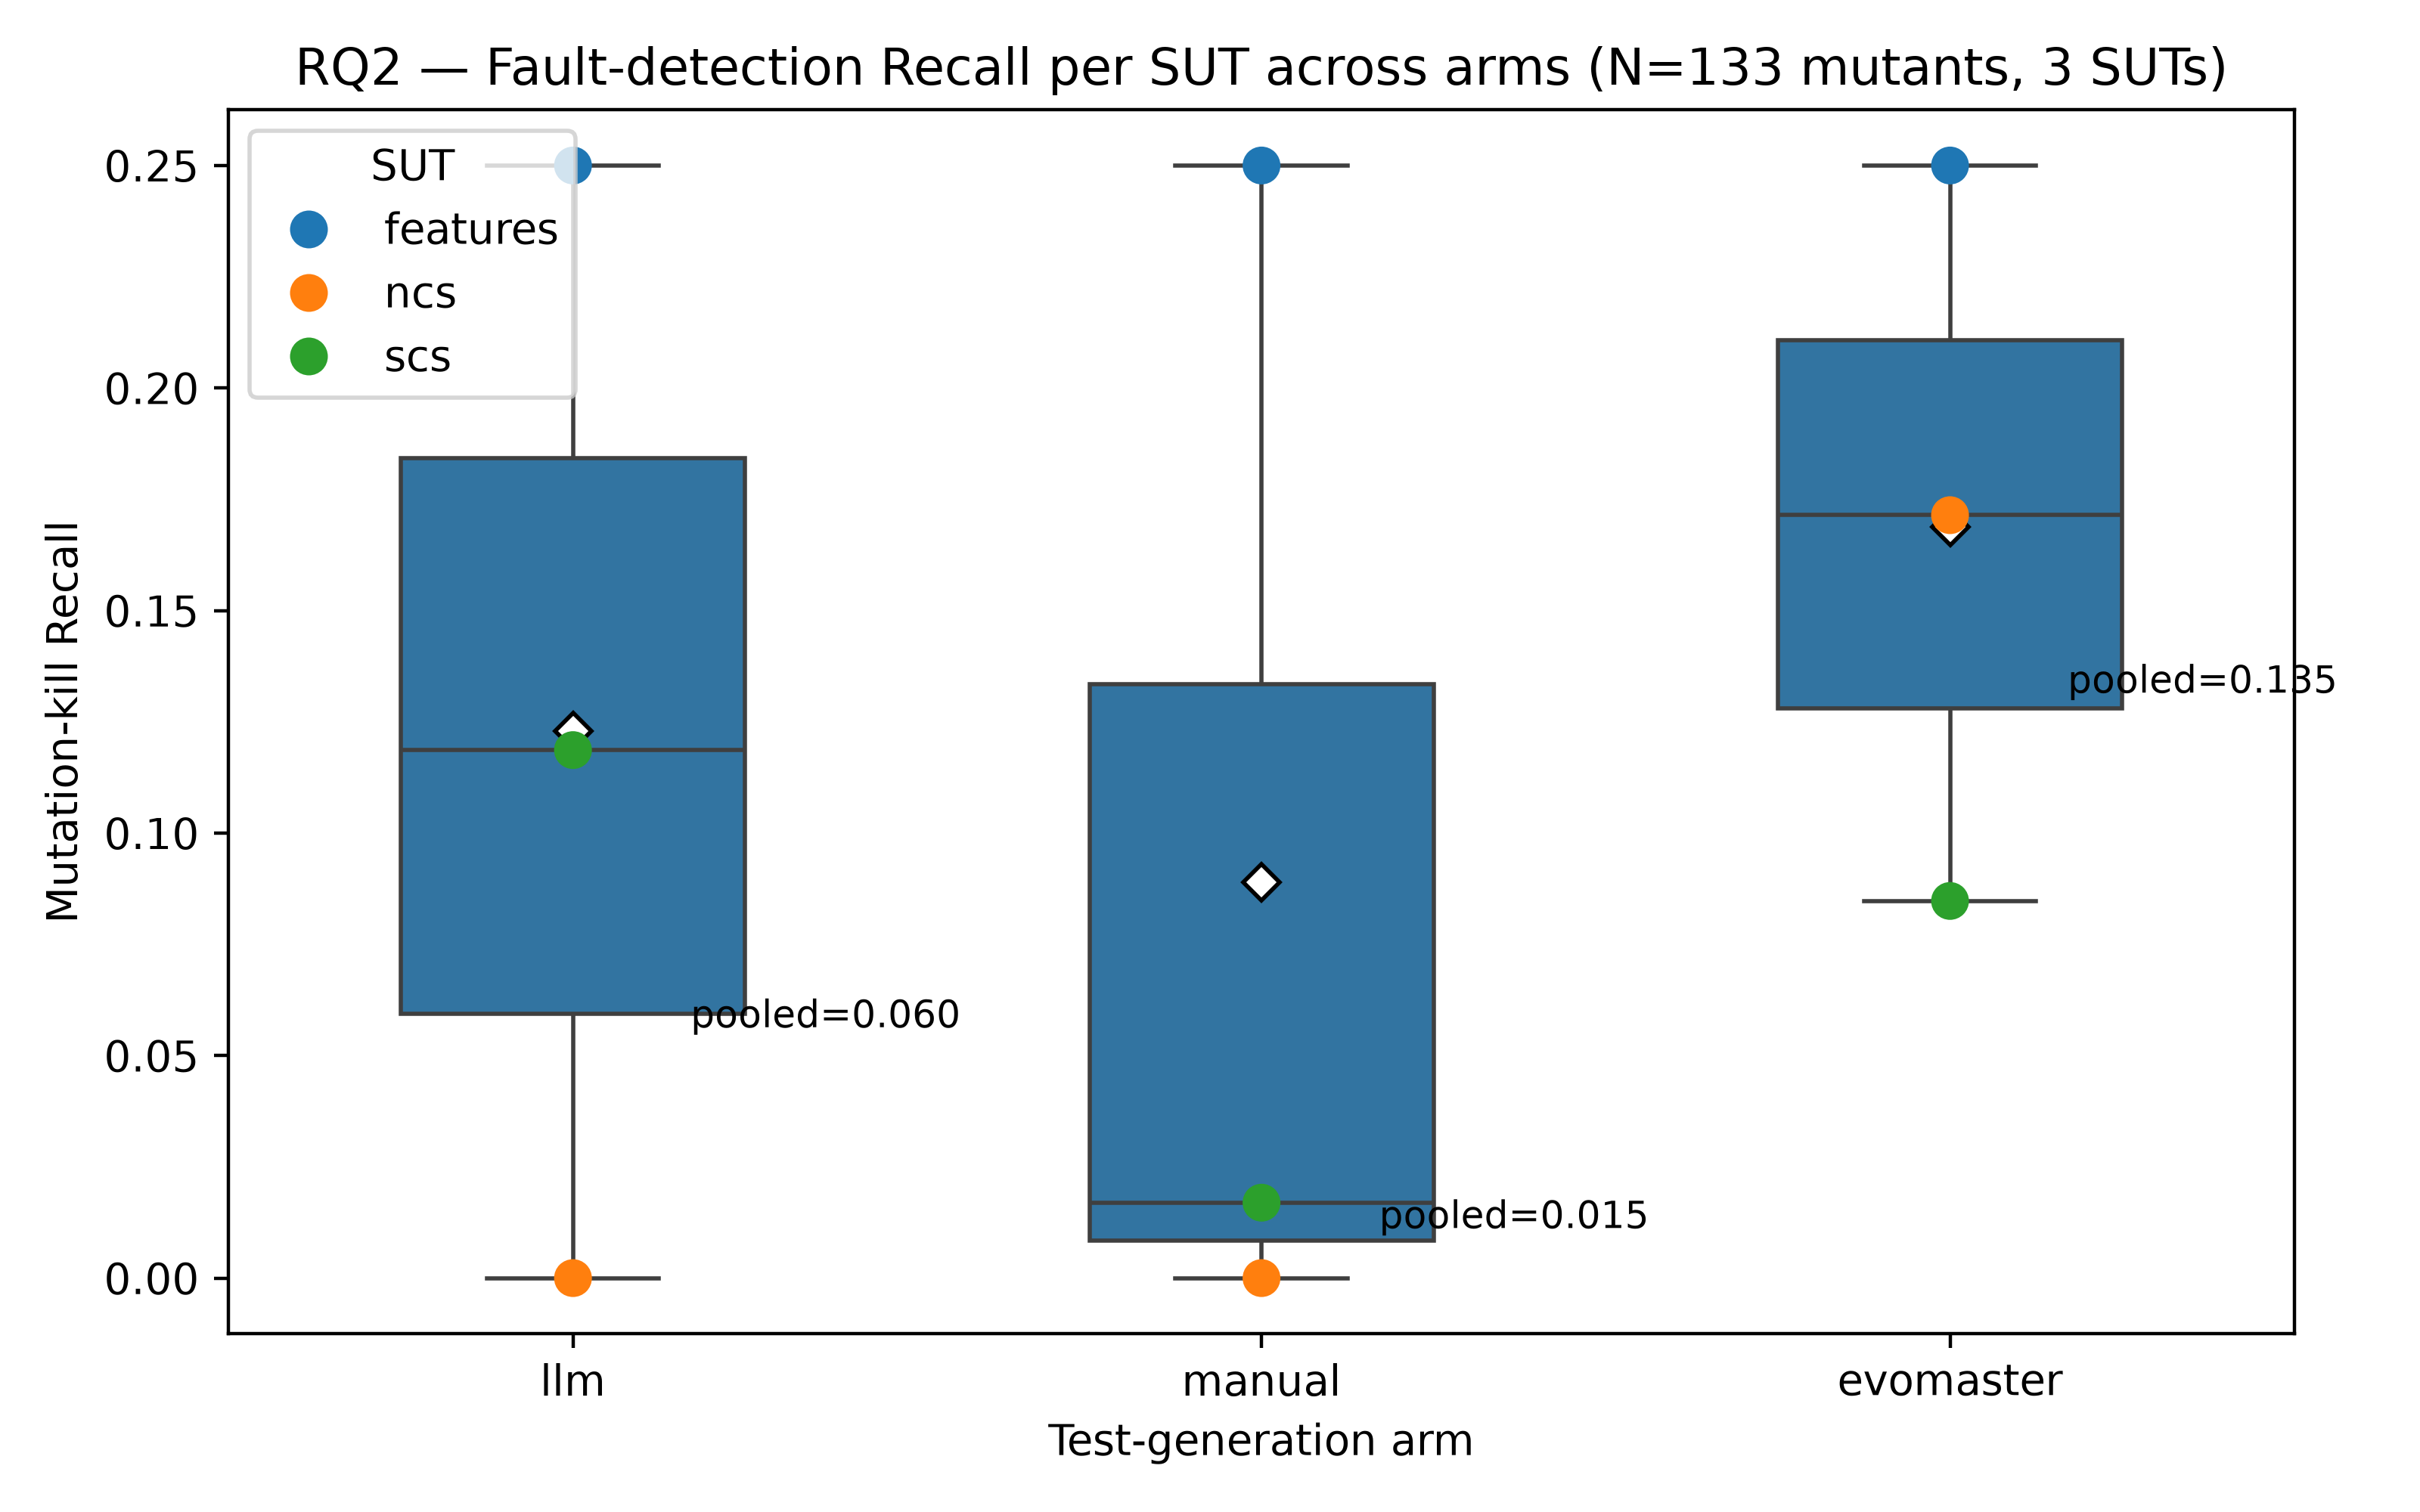
\includegraphics[width=\columnwidth]{fig1_distribution.png}
  \caption{RQ2 --- distribution of fault-detection Recall across the three arms over
  \RQIIn{} seeded faults. EvoMaster's advantage is concentrated on the arithmetic-heavy
  \texttt{rest-ncs} subject.}
  \label{fig:rq2}
\end{figure}

\begin{figure}[t]
  \centering
  
\includegraphics[width=\columnwidth]{fig2_comparison.png}
  \caption{RQ3 --- per-endpoint edge-case scenario counts, LLM versus manual across
  \RQIIIn{} operations. The LLM leads on \RQIIIpairsLlm{} operations, manual on
  \RQIIIpairsManual{}.}
  \label{fig:rq3}
\end{figure}

\section{Discussion}
\label{sec:discussion}

\subsection{Why volume and effectiveness came apart}

The headline of Section~\ref{sec:results} is a dissociation: the LLM produced
$\PDvolumeRatioLlmEvo\times$ EvoMaster's test volume, covered every operation, generated
\RQIIItotalLlm{} edge-case scenarios against manual's \RQIIItotalManual{}, and still killed
half as many faults. Treating this as a paradox is a mistake. It follows directly from
\emph{what kind of assertion each arm writes}.

The LLM reads an OpenAPI specification. A specification documents \emph{status codes}: this
path returns 200, that one 400 on bad input. Tests synthesised from it therefore assert on
the status code and, at best, on the shape of the response body --- an oracle of the form
``the response is in the plausible class for this request.'' Our manual EP/BVA suite, drawn
from the same specification, writes the same kind of assertion. Both are
\emph{specification-derived status oracles}.

Now consider what our mutants do. A relational or arithmetic operator replacement inside a
numerical routine --- \texttt{<} becoming \texttt{<=}, \texttt{/} becoming \texttt{*} ---
changes a \emph{computed value}. The endpoint still accepts the request, still runs to
completion, still returns 200. Only the number in the body is now wrong. A status oracle
cannot see this. The test passes on the mutant exactly as it passed on the original, and
the fault survives.

EvoMaster writes a different kind of oracle. Its black-box mode records the actual response
of the original system and emits assertions pinning those recorded values. That is a
\emph{regression oracle}: it fails whenever any observed value changes, whether or not the
status does. Against value-changing mutants this is precisely the right instrument.

So the arms were never measuring the same thing. The LLM and manual arms answer ``does the
API respond in the documented class?''; EvoMaster answers ``does the API still compute what
it computed before?'' Our fault population consists almost entirely of value faults, so it
interrogates the second question. EvoMaster's win is not evidence that search-based
generation is smarter than an LLM --- it is evidence that a regression oracle beats a status
oracle on value faults, which is close to a tautology once stated.

Three observations support this account over alternatives.

\textbf{The per-subject pattern matches the prediction.} If oracle kind drives the result,
EvoMaster's advantage should concentrate where faults are most value-like. It does:
EvoMaster leads decisively on \texttt{rest-ncs} (\RQIINcsEvo{} against \RQIINcsLlm{}), whose
controllers are numerical routines where nearly every mutant shifts a computed value while
preserving the status. On \texttt{rest-scs}, which has more string and validation logic and
so more mutants that flip a response \emph{class}, the LLM leads (\RQIIScsLlm{} against
\RQIIScsEvo{}). The ordering inverts with fault character, exactly as the mechanism
predicts, and not with anything about the generators' sophistication.

\textbf{The LLM wins where its oracle is adequate.} On the documented error surface --- where
being wrong \emph{means} returning a different status --- the LLM leads every arm,
triggering \PDerrTriggeredLlm{} of \PDerrKey{} error behaviours against manual's
\PDerrTriggeredManual{} and EvoMaster's \PDerrTriggeredEvo{}, and eliciting a genuine 500
crash. Where a status oracle suffices, the LLM's superior volume converts into superior
detection. Where it does not, volume buys nothing.

\textbf{The degenerate LLM-manual tie is the mechanism's signature.} Two arms with zero
discordant pairs over \RQIIn{} faults is a startling result, and the same-author confound
(Section~\ref{sec:results-degenerate}) is a genuine part of the explanation. But it cannot
be the whole of it, because both suites are also \emph{structurally} blind to the same fault
class: any two status-oracle suites, however independently authored, are constrained to miss
every value fault. Independent authorship would move which \emph{status-visible} faults each
catches; it would not let either see a wrong number behind a 200. We therefore expect an
independently authored manual suite to remain close to the LLM on this fault population ---
a prediction our design leaves testable rather than resolves, and we flag it as such rather
than presenting the tie as a finding.

\subsection{Implications}

\textbf{For practitioners.} An LLM generator is a strong \emph{breadth} instrument and a
weak \emph{depth} one. It will reach every documented operation and probe the documented
error surface harder than a human or a search tool. It will not notice that your pricing
routine now returns the wrong total, because nothing in your specification says what the
right total is. The actionable rule: use LLM generation for specification conformance and
error-path breadth; do not let it displace regression oracles, property-based assertions, or
example-based expected values on computational paths. The two are complements, and our data
say the complement is not optional --- half the detected faults came from the arm the LLM
would have replaced.

\textbf{For the field.} Every metric in our study that the surveyed literature actually uses
--- coverage, scenario counts, 500-error tallies --- ranked the LLM first. The ground truth
ranked it second. That is not a quirk of our subjects; it is a structural consequence of
scoring test suites on volume proxies. When AutoRestTest reports 42 server errors against
EvoMaster's 20~\cite{autoresttest}, or LlamaRestTest 204 faults against 130~\cite{llamaresttest},
those numbers are real but they measure \emph{how hard the documented error surface was
hit}, not \emph{what fraction of faults was found}. Our results show the two can order
arms oppositely on the same code. Per-endpoint scenario counts --- the metric GAP-M asks
for and which we introduce --- are subject to the same caveat, and we would rather say so
than let our own contribution be misread: RQ3 is a measure of what the LLM \emph{writes},
and Section~\ref{sec:results-pvd} shows how little that predicted about what it
\emph{caught}.

\textbf{For benchmark design.} The field needs pre-seeded-fault benchmarks not because
Recall is a nicer statistic, but because without a denominator these two orderings are
indistinguishable. We would additionally argue that a benchmark should stratify its fault
population by \emph{oracle-observability} --- status-visible versus value-only --- since our
results show that single axis reordering the arms. A benchmark of only value faults makes
regression-oracle tools look dominant; one of only status faults makes LLMs look dominant.
Neither is a fact about the generators.

\subsection{Why the low absolute Recall is informative}

All three arms score low in absolute terms: the best, EvoMaster, kills \PDkilledEvo{} of
\PDkilledTotal{} mutants (\RQIIrecallEvoPct\%). We report this rather than tuning it away,
because it is a finding about black-box REST testing rather than a defect in our setup. Our
mutants live in core logic reachable only through the HTTP contract, and many are
\emph{equivalent-at-the-boundary}: the value they corrupt never surfaces in a response
field, or surfaces only for inputs no arm generated. A white-box tool with code-coverage
feedback would score higher. The honest reading is that black-box REST suites --- LLM,
human, or search-based --- detect a small minority of seeded logic faults, and the
interesting question is not which arm wins a low-scoring race but which fault classes all
three systematically cannot see.

\section{Threats to Validity}
\label{sec:threats}

\subsection{Construct validity}

\textbf{The manual arm is independent-agent, not independent-human.} Our proposal specified
an independent human baseline. No human cohort was available, so the manual suite was
re-authored by a \emph{separate, isolated} model session with no shared context with the LLM
suite --- spec-only input, blind to the LLM output and to the fault catalog. This resolves
the pilot's same-author confound (there, one session wrote both suites, and they killed
identical mutant sets); with the suites separated, the LLM-versus-manual comparison becomes
live and the arms diverge ($b=\RQIImcnemarLMb$, $c=\RQIImcnemarLMc$;
Section~\ref{sec:results-rq2}). What remains uncontrolled is the gap between an
\emph{independent agent} and an \emph{independent human tester}: a human cohort might bring
domain intuition an EP/BVA-from-spec agent lacks, and could plausibly close some of the LLM's
lead. We therefore state the RQ2 manual result as ``LLM versus an independently authored,
specification-derived EP/BVA suite,'' not ``LLM versus human testers,'' and flag the
human-cohort replication as the highest-value next step. The RQ2 conclusion is unaffected by
this caveat in \emph{direction}: the LLM's kills are a superset of the manual suite's, so no
plausible relabelling of the baseline reverses the sign.

\textbf{The LLM-versus-EvoMaster significance hinges on one boundary mutant.} We disclose
this prominently. Our re-execution reproduces the pilot's EvoMaster kills exactly (identical
12 mutants on \texttt{rest-ncs}) and the LLM's \texttt{rest-scs} kills exactly, but on
\texttt{rest-ncs} the LLM's Recall falls from the pilot's 1/70 to \RQIINcsLlm{}: one LLM test
exercising \texttt{bessj} at the boundary $n=2$ passed on the pilot's build of the original
SUT but fails on our clean rebuild, so it is excluded as an invalid oracle and no longer
kills that mutant. Bessel-function evaluation at the boundary is numerically sensitive, and
this is a genuine reproduction limit rather than a pipeline error (the exact EvoMaster match
rules out a build fault). Its effect is to shift the LLM-versus-EvoMaster discordant count
from six to $\RQIImcnemarLEb$, which is what carries the McNemar $p$ across the
$\alpha=\alphaRaw$ threshold --- from just above it in the pilot to $\RQIImcnemarLEp$ here.
The \emph{direction} (EvoMaster $>$ LLM) is robust either way; the $\alpha=\alphaRaw$ verdict
is not, and should be read as ``EvoMaster leads, at the edge of significance'' rather than as
a firm rejection.

\textbf{Oracle strength differs across arms by construction.} EvoMaster's recorded-value
regression oracles are strictly stronger on value faults than the spec-derived status
oracles of the LLM and manual arms. This is not a flaw we failed to control --- it is the
independent variable that Section~\ref{sec:discussion} identifies as driving the result ---
but it does mean RQ2 does not compare ``generation techniques'' with oracle strength held
constant. A fairer isolation of generation quality would fix the oracle kind across arms and
vary only the generator. We report kill-by-subject so the interaction is visible rather than
hidden in a pooled average.

\textbf{Mutation kills are a proxy for real faults.} We use standard PIT/Offutt operator
families~\cite{pit,offutt} to keep the population conventional, but a seeded single-token
mutation is not a field defect. Coverage is likewise a proxy for test quality. We report
Recall, coverage, and edge-case counts jointly, and Section~\ref{sec:results-pvd} exists
precisely because any one of them alone gives the wrong ranking.

\subsection{Internal validity}

\textbf{Equivalent mutants are not excluded.} We do not attempt to identify semantically
equivalent mutants, which is undecidable in general. Some fraction of the \RQIIn{} mutants
may be unkillable by \emph{any} black-box suite, which deflates all three arms' Recall
uniformly. This weakens the absolute figures but not the comparison, since every arm faces
the identical population.

\textbf{LLM non-determinism.} Generation used temperature 0 and a fixed seed, and raw
outputs are frozen in the repository, but LLM sampling is not bit-reproducible across
provider-side model updates. The generated suites are committed, so the analysis is
reproducible even if regeneration is not.

\textbf{Mutation confined to controller and core-logic classes.} We seed where faults are
observable through the HTTP contract. Faults in configuration, persistence, or serialisation
layers are out of the population and out of our conclusions.

\subsection{External validity}

\textbf{Three JVM APIs, \RQIopsTotal{} operations.} Our subjects are small EMB services. The
findings are ``EMB-only, JVM-only'' and should not be read as covering large production APIs,
authenticated flows, or non-JVM stacks. The \texttt{user-management} service (MySQL-backed)
was excluded on setup cost, which leaves authentication endpoints under-represented --- a
real gap, since RQ1's miss profile cannot speak to the endpoint type most likely to be
missed.

\textbf{The \texttt{features-service} imbalance.} That subject contributes 4 mutants against
70 and 59 for the others, because its controllers contain little arithmetic to mutate. All
three arms tie there (\RQIIFeaturesLlm{} each), so it contributes almost nothing to the
pooled comparison. We report it rather than dropping it, as dropping a subject after seeing
its results would be HARKing-adjacent.

\textbf{One LLM, one configuration.} Claude Sonnet 4.6 at temperature 0 with one frozen
prompt. Our results do not generalise to the GPT family that dominates the literature
(Section~\ref{sec:related}), to open-source models, or to agentic multi-turn strategies.
Since we identify \emph{oracle kind} rather than model capability as the mechanism, we would
expect the qualitative finding to hold for any spec-only generator --- but that is a
prediction, not a result.

\subsection{Conclusion validity}

\textbf{The Friedman test is underpowered by design.} With $n=3$ subjects it cannot detect
realistic effects ($\chi^2=\RQIIfriedmanChi$, $p=\RQIIfriedmanP$), which is why the proposal
pre-designated the pooled per-fault McNemar test ($N=\RQIIn$) as the primary RQ2 analysis
rather than promoting it after the omnibus test failed.

\textbf{RQ2's pairwise tests are significant but fragile.} Both McNemar comparisons reject at
$\alpha=\alphaRaw$ ($p=\RQIImcnemarLEp$ for LLM-versus-EvoMaster, $p=\RQIImcnemarLMp$ for
LLM-versus-manual), but neither clears the Bonferroni threshold $\alphaBonf$, and approximate
achieved power for the EvoMaster comparison is only \RQIImcnemarLEpower{} --- below
conventional adequacy. We therefore rest the RQ2 conclusions on the \emph{direction and
effect size} (EvoMaster's kills strictly dominate on value faults; the LLM's kills strictly
contain the manual suite's) rather than on the $p$-values alone, and we do not upgrade
``significant at $\alphaRaw$'' to ``firmly established.'' The power figure is itself an
approximation: statsmodels has no exact McNemar power routine, so we substitute a
two-independent-proportion calculation on the same proportions, disclosed in
\texttt{summary.json} alongside the value.

\textbf{Multiplicity.} Three RQ families are tested. We apply Holm correction within RQ2's
post-hoc comparisons and report a Bonferroni threshold across families
($\alpha_{\text{adj}}\approx\alphaBonf$). RQ1 and RQ3 survive both comfortably
($p=\RQIpvalue$ and $p=\RQIIIpvalue$); the RQ2 pairwise tests survive the raw threshold but
not Bonferroni, which is why we read them as directional evidence rather than as decisive
rejections.

\section{Conclusion}
\label{sec:conclusion}

We ran the comparison the REST-API-testing literature has not: an LLM generator, a manual
EP/BVA suite, and EvoMaster, on the same three APIs, against a \emph{known} population of
\RQIIn{} seeded faults rather than a tally of errors observed on a live system.

The answer to ``can an LLM out-test a human baseline and a search-based tool'' is: it
out-tests the human-style baseline and is out-tested by the tool. On every metric the field
currently reports, the LLM leads both: \RQIcoveragePct\% endpoint coverage ($p=\RQIpvalue$),
\RQIIItotalLlm{} edge-case scenarios against \RQIIItotalManual{} ($p=\RQIIIpvalue$,
rank-biserial $\RQIIIrankBiserial$), \PDtestsLlm{} test cases to EvoMaster's \PDtestsEvo{},
and \PDerrTriggeredLlm{} of \PDerrKey{} documented HTTP error behaviours triggered. On the
ground truth the ordering is EvoMaster \RQIIrecallEvo{} $>$ LLM \RQIIrecallLlm{} $>$ manual
\RQIIrecallManual{}: the LLM significantly out-detects an independently authored EP/BVA suite
($p=\RQIImcnemarLMp$, its kills a strict superset), yet is itself out-detected by EvoMaster
($p=\RQIImcnemarLEp$; both at the raw threshold, neither under Bonferroni, so directional
rather than decisive).

The explanation is not about model capability. A generator that reads a specification writes
assertions about \emph{status codes}, and a fault that changes a computed value while leaving
the status intact is invisible to every such assertion, no matter how many are written.
EvoMaster's recorded-value regression oracles see exactly those faults. The evidence is that
the arms' ordering tracks fault character rather than generator sophistication: on the
arithmetic-heavy \texttt{rest-ncs} \emph{both} status-oracle arms score \RQIINcsLlm{} while
EvoMaster kills \RQIINcsEvo{}; on the validation-heavy \texttt{rest-scs} the LLM leads every
arm. Two levels compose: oracle \emph{kind} fixes the ceiling (status oracles cannot reach
EvoMaster on value faults), and within a kind, \emph{volume} decides how much of the
reachable fault set is caught --- which is why the LLM's \PDtestsLlm{} tests beat the leaner
independent manual's \PDtestsManual{} where the faults are status-visible.

Three consequences follow. For practitioners, LLM generation is a breadth instrument that
complements rather than replaces value-based oracles --- it beats a human-style suite yet
still missed more than half the faults EvoMaster's regression oracles caught. For the field,
the metric that ranks the LLM first over EvoMaster (volume) and the metric that ranks it
below (ground-truth Recall) disagree on the same code, so the comparative claims currently in
the literature are not measuring what their framing implies. For benchmark design, fault
populations should be stratified by oracle-observability, because that single axis reorders
the arms.

Our principal remaining limitation is that the independent manual baseline is an isolated
\emph{agent} session, not a human cohort; a human replication against the same \RQIIn{}
mutants is the highest-value next step, and our pipeline runs it without modification. Beyond
it, the natural studies are an oracle-controlled comparison that fixes assertion kind and
varies only the generator, a fault population stratified by oracle-observability, and the
GAP-T ablation across model families. The pipeline, prompts, fault catalogs, and raw data are
committed, and every number above regenerates from them by script.


% =====================================================================
% ACTION REQUIRED BEFORE SUBMISSION
% This section states, on the authors' behalf, how AI tools were used.
% Springer requires that such use be disclosed and that LLMs are NOT
% listed as authors. The text below describes the uses visible in the
% repository. VERIFY EVERY SENTENCE against what the team actually did
% and edit it to match; an inaccurate disclosure is worse than none.
% =====================================================================

\section*{Use of AI Tools}
\label{sec:ai-disclosure}

This study concerns LLM-based test generation, so we separate three distinct roles that
language models play in it.

\textbf{As an object of study.} Claude Sonnet 4.6 is the subject of the LLM arm. Its
configuration, prompt and outputs are specified in Section~\ref{sec:method} and committed to
the replication package.

\textbf{As an instrument in the experiment.} The manual EP/BVA arm was authored by a separate,
isolated model session rather than by a human cohort, because no human cohort was available.
We treat this as a construct-validity threat, label the arm ``independently authored'' rather
than ``human'' throughout, and discuss its consequences in Section~\ref{sec:threats}.

\textbf{In manuscript preparation.} The authors used an LLM assistant to draft and edit prose,
and to convert the manuscript to this template. All research design, experimental execution,
data analysis and interpretation were carried out by the authors. Every computed statistic
reported here is generated from committed raw data by \texttt{scripts/gen\_paper\_macros.py}
and was not written by a model or transcribed by hand (Section~\ref{sec:method-repro}). The
authors read,
verified and take full responsibility for the entire content of this paper. No LLM is listed
as an author, in line with Springer's authorship policy.

\section*{Data Availability}

The replication package contains the mutation catalogs, the generated test suites for all
three arms, the raw kill matrices, the analysis scripts and the notebook that regenerates
every statistic in this paper. Subjects are drawn from the EvoMaster Benchmark (EMB,
LGPL-3.0); the upstream commit used is recorded in the repository.

% LNCS requires Disclosure of Interests in the `credits' environment, using the
% \discintname macro for the run-in heading (llncsdoc v2.26 sec. 5). It is mandatory,
% and must sit immediately before the bibliography.
\begin{credits}
\subsubsection{\discintname}
The authors have no competing interests to declare that are relevant to the content of this
article.
\end{credits}


\bibliographystyle{splncs04}
\bibliography{references}

\end{document}
